\documentclass[conference]{IEEEtran}
\usepackage{float}
\usepackage{cite}
\usepackage{graphicx}
\usepackage{url}
\usepackage{amsmath}
\usepackage{booktabs}
\graphicspath{{./}}
\usepackage{listings}
\usepackage{xcolor}
\definecolor{codegray}{gray}{0.95}
\lstset{
  backgroundcolor=\color{codegray},
  basicstyle=\ttfamily\footnotesize,
  frame=single,
  breaklines=true,
  captionpos=b,
  language=Java  % fallback to Java-style formatting
}


\title{Security Under Siege: A Comprehensive Analysis of Exploits and Defense Mechanisms in Decentralized Finance (DeFi)}

\author{\IEEEauthorblockN{ZAKI ABADI BIN PUTEH and MARSHITAH BINTI MAZLAN}
\IEEEauthorblockA{Department of Information Systems\\
Hanyang University Seoul, South Korea \\
zakotto@hanyang.ac.kr, marshi29@hanyang.ac.kr}}

\usepackage{tikz}
\usetikzlibrary{arrows.meta, positioning}

\begin{document}

\maketitle

\begin{abstract}
Decentralized Finance (DeFi) is revolutionizing financial ecosystems through transparent and permissionless systems powered by blockchain smart contracts. However, this autonomy comes with significant security risks. This paper offers a comprehensive survey of critical vulnerabilities within DeFi protocols, classifying them into flash loan exploits, oracle manipulations, reentrancy attacks, and Miner Extractable Value (MEV). We analyze over five major exploit case studies between 2020–2023, detailing attacker techniques and financial impacts. Further, we explore state-of-the-art mitigation strategies, including formal verification, zk-SNARKs, governance mechanisms, and decentralized insurance. Our findings aim to bridge the gap between protocol innovation and robust security design.
\end{abstract}

\begin{IEEEkeywords}
DeFi, smart contracts, blockchain, security, flash loan, oracle manipulation, reentrancy, decentralized finance
\end{IEEEkeywords}

\section{Introduction}
Decentralized Finance (DeFi) encompasses financial services on blockchain platforms, mainly Ethereum, providing decentralized lending, asset management, and trading without centralized intermediaries. Smart contracts automate these operations, significantly reducing operational costs and increasing transparency. Nevertheless, vulnerabilities inherent in smart contracts have led to substantial financial losses. Analyzing these vulnerabilities is essential to enhance the security posture of the DeFi ecosystem.
This paper makes the following contributions:
\begin{itemize}
  \item Presents a taxonomy of DeFi vulnerabilities across four main classes.
  \item Provides in-depth analysis of five high-impact DeFi exploits from 2020 to 2023.
  \item Evaluates mitigation strategies including smart contract audits, formal methods, and decentralized insurance.
  \item Identifies research gaps and future security directions such as regulatory-compliant DeFi and zero-knowledge defenses.
\end{itemize}


\section{DeFi Background}

Decentralized Finance (DeFi) refers to a new financial ecosystem built on blockchain technology that eliminates the need for traditional financial intermediaries such as banks, brokers, or payment processors. Instead, DeFi protocols operate through smart contracts—self-executing pieces of code deployed on blockchain networks like Ethereum—that automatically enforce rules and execute transactions without human intervention.

At its core, DeFi enables anyone with an internet connection and a digital wallet to access financial services such as lending, borrowing, trading, insurance, and asset management in a permissionless manner. This openness contrasts sharply with traditional finance, where access is often controlled by centralized institutions and regulated environments.

Key components of the DeFi stack include:
\begin{itemize}
  \item \textbf{Decentralized Exchanges (DEXs)}: Platforms like Uniswap and SushiSwap allow users to trade tokens directly with each other using liquidity pools, rather than through centralized order books.
  \item \textbf{Lending and Borrowing Protocols}: Platforms such as Aave and Compound enable users to lend assets and earn interest or borrow assets by posting collateral, all governed by smart contracts.
  \item \textbf{Stablecoins}: Cryptocurrencies like DAI or USDC are designed to maintain a stable value relative to fiat currencies and serve as key instruments in many DeFi applications.
  \item \textbf{Oracles}: Networks like Chainlink provide external (off-chain) data, such as real-time asset prices, to smart contracts, enabling them to interact meaningfully with real-world events.
\end{itemize}

Smart contracts in DeFi are typically immutable once deployed, meaning their code cannot be changed unless pre-programmed upgradability is built in. This immutability provides transparency and trust but also introduces significant risks. Even minor programming errors or unintended interactions between protocols can be exploited, resulting in major financial losses. As DeFi protocols often “compose” or build on top of one another like Lego blocks, a vulnerability in one contract can cascade across multiple systems.

In summary, DeFi represents a revolutionary shift in how financial services are created, accessed, and managed—but it also introduces a unique set of technical and economic risks that must be carefully understood.



\section{Related Work}
Recent research has investigated the increasing vulnerability of DeFi platforms to sophisticated attacks. Master et al. (2025) introduced the DMind Benchmark to evaluate LLM capabilities for security diagnostics in the Web3 domain~\cite{master2025dmind}. Zhao et al. (2025) explored Distributed Transaction Sequencing as a mitigation strategy for blockchain extractable value (BEV)~\cite{zhao2025mitigating}. Wu (2024) proposed static analysis techniques for detecting flash loan vulnerabilities~\cite{wu2024static}.

Rahnama (2025) designed DeFiSentinel, an AI-enhanced architecture for anomaly detection in smart contracts~\cite{rahnama2025defisentinel}. Zhang et al. (2024) presented TransFront, a novel model to detect front-running attacks using bi-path fusion~\cite{zhang2024transfront}. Hegde and Hegde (2024) discussed practical implementations of transparent blockchain systems in finance~\cite{hegde2024efficient}.

These works underscore the importance of not just identifying vulnerabilities but also embedding defensive layers into DeFi protocol design, a direction further extended by our survey.

\section{Common Vulnerabilities}

Decentralized Finance (DeFi) systems rely heavily on smart contracts—automated programs that handle money on the blockchain. However, even small flaws in these smart contracts or how they interact with each other can be exploited by attackers. Below are some of the most common and dangerous types of attacks in the DeFi space.


\subsection{Flash Loan Attacks}

Flash loans are a special type of loan in DeFi that allow users to borrow large amounts of cryptocurrency instantly—without providing any collateral—as long as the loan is repaid within the same transaction block. Think of it like borrowing \$1 million for just one second, using it, and giving it back before the transaction completes.

Attackers exploit flash loans by temporarily manipulating market conditions. For example, they may inflate or deflate the price of a token on a decentralized exchange (DEX), deceive a smart contract into believing a token is worth more than it actually is, and then extract value based on that false information. All of this occurs in a single atomic transaction.

As illustrated in Figure~\ref{fig:flashloan_tikz}, a typical flash loan exploit follows a precise flow: the attacker initiates the loan, manipulates prices via DEXs or oracles, triggers a vulnerable contract, profits from the exploit, and finally repays the loan within the same transaction. A real-world example of such an attack occurred in the bZx protocol, where multiple flash loan exploits led to the loss of millions of dollars.

\begin{figure}[H]
\centering
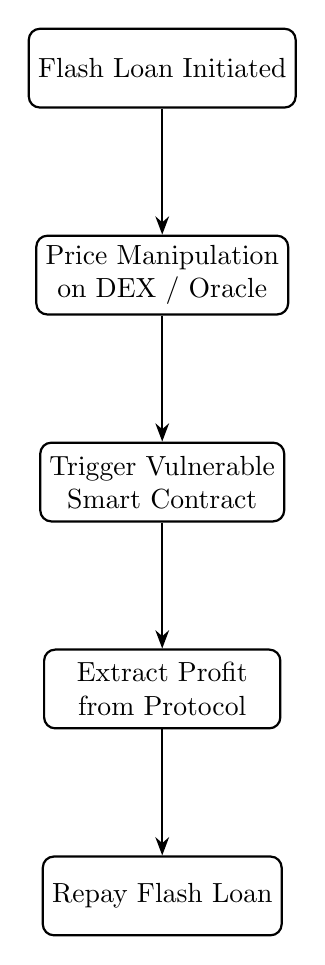
\begin{tikzpicture}[
  node distance=1.6cm and 2.4cm,
  every node/.style={draw, align=center, rounded corners, minimum width=3cm, minimum height=1cm},
  every path/.style={->, thick, >=Stealth}
]

\node (start) {Flash Loan Initiated};
\node (manip) [below=of start] {Price Manipulation \\ on DEX / Oracle};
\node (trigger) [below=of manip] {Trigger Vulnerable \\ Smart Contract};
\node (profit) [below=of trigger] {Extract Profit \\ from Protocol};
\node (repay) [below=of profit] {Repay Flash Loan};

\draw (start) -- (manip);
\draw (manip) -- (trigger);
\draw (trigger) -- (profit);
\draw (profit) -- (repay);

\end{tikzpicture}
\caption{Flash loan exploit flow in a DeFi attack scenario.}
\label{fig:flashloan_tikz}
\end{figure}

\subsection{Oracle Manipulation}

Smart contracts can't access real-world information (like token prices) by themselves. They depend on “oracles” to feed them this data. Oracles are like messengers that tell smart contracts things like the price of Ethereum or Bitcoin.

But if the oracle gets its information from a weak source—such as a small or thinly-traded DEX—attackers can trick it. For instance, in the Mango Markets exploit, attackers made it look like their token was worth far more than it really was. The smart contract believed the fake price and allowed them to borrow massive amounts of money, which they never intended to repay.

\subsection{Reentrancy Attacks}

A reentrancy attack is like a sneaky backdoor call. Imagine a smart contract that lets users withdraw funds. It first sends money to the user, then updates the balance. In a reentrancy attack, the attacker writes another smart contract that interrupts this process, calling the vulnerable contract again before the balance gets updated.

This trick allows the attacker to withdraw money multiple times in one go. The most famous example is the DAO hack in 2016, where about \$60 million was stolen using this technique. This type of bug still exists today in poorly written contracts.

\begin{figure}[H]
\begin{lstlisting}[caption=Simplified vulnerable contract in Solidity]
pragma solidity ^0.8.0;

contract VulnerableBank {
    mapping(address => uint256) public balances;

    function deposit() public payable {
        balances[msg.sender] += msg.value;
    }

    function withdraw(uint256 amount) public {
        require(balances[msg.sender] >= amount, "Insufficient balance");

        // Sends ETH to user
        (bool success, ) = msg.sender.call{value: amount}("");
        require(success, "Transfer failed");

        // Updates balance AFTER sending
        balances[msg.sender] -= amount;
    }
}
\end{lstlisting}
\end{figure}

In the above contract, the `withdraw()` function sends ETH to the caller and then updates the internal balance. This sequence opens up a reentrancy vulnerability: if the caller is a malicious contract with a fallback function that re-calls `withdraw()` before the balance is updated, it can recursively drain funds. The attack exploits the fact that Ethereum allows external calls to arbitrary contracts, which can trigger unexpected control flow.

\textbf{Fix:} To mitigate this, always update the state (e.g., subtract balance) \emph{before} making external calls, or use built-in mutexes (like OpenZeppelin's `ReentrancyGuard`).

\subsection{Front-Running and Miner Extractable Value (MEV)}

In traditional finance, “front-running” is when someone sees a big order coming in and jumps ahead to profit from it. In DeFi, this happens when miners or bots rearrange the order of transactions in the block they're confirming. 

This practice, known as Miner Extractable Value (MEV), allows them to make money by exploiting price changes between transactions. For example, if someone is swapping tokens on a DEX, a bot might insert its own trade right before and right after to make a profit—at the user's expense. This creates unfair conditions and has become a growing problem.

Researchers and developers are exploring solutions like “private transaction pools” (where bots can't see your transaction) and “fair transaction ordering” to reduce MEV risks.

\begin{table}[H]
\caption{Comparison of Common DeFi Vulnerabilities}
\centering
\begin{tabular}{@{}p{2.5cm}p{4.5cm}p{1.6cm}@{}}
\toprule
\textbf{Vulnerability} & \textbf{Core Idea} & \textbf{Impact Level} \\
\midrule
Flash Loan Attacks & Exploit atomic, uncollateralized loans to manipulate on-chain state within a single transaction & High \\
Oracle Manipulation & Feed manipulated price data to smart contracts via weak oracles or illiquid markets & High \\
Reentrancy Attacks & Repeatedly call back into a vulnerable function before it finishes execution & Medium–High \\
Miner Extractable Value (MEV) & Reorder or insert transactions to profit from user trades or arbitrage opportunities & Medium \\
\bottomrule
\end{tabular}
\label{tab:vulnerability_comparison}
\end{table}


\section{Detailed Case Studies}

\subsection{bZx Protocol (2020)}
bZx experienced multiple flash loan exploits involving market manipulations and oracle discrepancies. Attackers leveraged liquidity pool imbalances to drain approximately \$8 million, underscoring critical vulnerabilities in flash loan mechanics.

\subsection{Cream Finance (2021)}
Cream Finance suffered a sophisticated reentrancy exploit, with attackers executing flash loan-enabled double-spending, ultimately resulting in losses exceeding \$130 million.

\subsection{Euler Finance (2023)}
Euler Finance encountered a logic vulnerability exploit in its liquidity management contract, resulting in a significant \$197 million loss. Eventually, these funds were largely recovered due to public and legal pressure.

\subsection{Mango Markets (2022)}
Attackers exploited thin liquidity and manipulated token pricing on Mango Markets to artificially increase collateral value, enabling a theft of around \$117 million. This highlighted critical weaknesses in oracle reliability.

\subsection{Harvest Finance (2020)}
Harvest Finance experienced a flash loan attack manipulating liquidity pool calculations, resulting in a loss of around \$24 million. This demonstrated the complexity and risk associated with DeFi protocol interactions.

\begin{table}[htbp]
\caption{Major DeFi Exploits}
\centering
\begin{tabular}{@{}llll@{}}
\toprule
\textbf{Protocol} & \textbf{Year} & \textbf{Attack Type} & \textbf{Loss} \\
\midrule
bZx & 2020 & Flash Loan & \$8M \\
Cream Finance & 2021 & Reentrancy & \$130M \\
Euler Finance & 2023 & Logic Exploit & \$197M \\
Mango Markets & 2022 & Oracle Manipulation & \$117M \\
Harvest Finance & 2020 & Flash Loan & \$24M \\
\bottomrule
\end{tabular}
\end{table}

\section{Defensive Measures}
Considering how quickly the DeFi threat environment is changing, protecting smart contracts and protocols requires a multipronged strategy.  Below, we look at well-known mitigation techniques, their advantages and disadvantages, and new advancements that address pressing issues.

\subsection{Auditing and Formal Verification}

In decentralized finance (DeFi), smart contracts often manage millions of dollars and cannot be changed once deployed. A small bug can lead to massive losses. To prevent this, formal verification is used as a powerful security method. It works by using math and logic to check that the code will always behave correctly under all possible conditions—not just some test cases \cite{certora2023blog}.

\usetikzlibrary{shapes.geometric, arrows, positioning}
\begin{figure}[H]
\centering
\begin{tikzpicture}[
  node distance=0.6cm and 1.5cm,
  every node/.style={
    draw,
    align=center,
    rounded corners,
    minimum width=1cm,
    minimum height=0.4cm,
    font=\tiny
  },
  every path/.style={->, line width=0.5pt, >=Stealth}
]

% Nodes
\node (start) {SC \\ Deploy};
\node (formal) [below=of start] {Formal \\ Verify};
\node (specs) [right=of formal] {Write \\ Specs};
\node (autoCheck) [below=of formal] {Auto \\ Checker};
\node (result) [below=of autoCheck, shape=diamond, aspect=2, draw, fill=green!30, minimum width=1.2cm, minimum height=1cm] {OK?};
\node (manualAudit) [left=of result] {Manual \\ Audit};
\node (deploy) [below=of result, yshift=-1cm] {Deploy};
\node (vulnerable) [right=of result] {Bug \\ Fix};

% Arrows
\draw (start) -- (formal);
\draw (formal) -- (autoCheck);
\draw (specs) -- (autoCheck);
\draw (autoCheck) -- (result);
\draw (result) -- node[above, font=\tiny] {Yes} (deploy);
\draw (result) -- node[above, font=\tiny] {No} (vulnerable);
\draw (vulnerable) |- (manualAudit);
\draw (manualAudit) |- (formal);

\end{tikzpicture}
\caption{Auditing \& Formal Verification Workflow}
\label{fig:audit-formal-verification}
\end{figure}



Unlike regular testing or manual audits, formal verification can prove key properties like no reentrancy or correct balance updates with certainty. Tools like the Certora Prover let developers write custom rules (called specifications) and then automatically check if the contract code follows them \cite{certora2024docs, szalachowski2021defioracles}.

Major DeFi platforms like Aave and Uniswap v4 use formal verification to protect important contract logic. Aave even includes it in its continuous integration system to check smart contract changes in real time \cite{certora2023blog}. Uniswap v4 applied it to verify key behaviors in areas like flash loans and hooks.

While formal verification doesn’t replace traditional audits or fuzz testing, it adds a deeper layer of protection by proving that critical rules always hold. This combination makes DeFi protocols more secure and resilient to complex attacks \cite{trailofbits2022ecosystem, openzeppelin2023audits}.

\subsection{Bug Bounties}

\sloppy Bug bounty programs invite independent security researchers often called “ethical hackers”—to find and responsibly disclose vulnerabilities in DeFi smart contracts. Projects offer monetary rewards based on the bug’s severity, encouraging external experts to hunt for weaknesses before malicious actors can exploit them \cite{cointracker_bugbounty}.


This crowdsourced strategy provides several key benefits:

\begin{itemize}
    \item \textbf{Broader coverage and fresh eyes.} By opening security to a global community, bounty programs uncover hidden issues that internal teams or audits might miss \cite{marcavage2023predicting, streamflow_defi_security}.
    \item \textbf{Continuous vigilance.} DeFi systems often change or expand; bounty programs offer a continuous safety net rather than a one-off review \cite{securrtech_loop}.
    \item \textbf{Cost-effective and scalable.} It’s often cheaper than hiring full-time security staff, and payments are issued only when valuable vulnerabilities are found \cite{consensys_bugbounty}.
    \item \textbf{Quick response.} Once a bug is reported, teams can fix issues swiftly, preventing financial loss and reinforcing user confidence \cite{coinmetro_crypto_bounties, streamflow_defi_security}.
\end{itemize}

Figure~\ref{fig:bugbountyflow} illustrates a typical workflow of a DeFi bug bounty system.

\begin{figure}[h!]
\centering
\resizebox{\linewidth}{!}{%
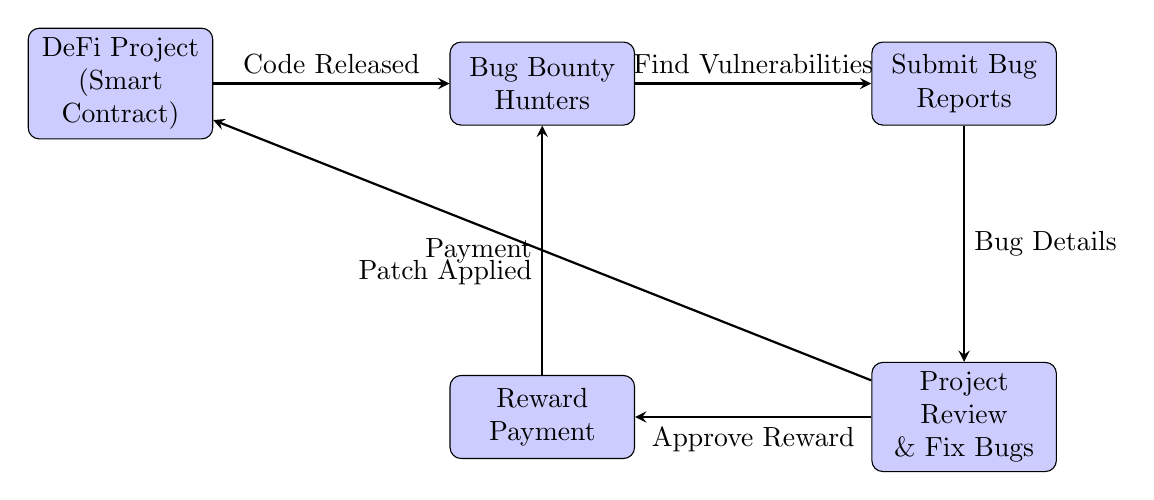
\begin{tikzpicture}[node distance=3cm, auto]
\tikzstyle{block} = [rectangle, draw, fill=blue!20, 
    text width=6em, text centered, rounded corners, minimum height=3em]
\tikzstyle{arrow} = [thick,->,>=stealth]

% Nodes
\node [block] (project) {DeFi Project \\ (Smart Contract)};
\node [block, right=of project] (hunters) {Bug Bounty Hunters};
\node [block, right=of hunters] (report) {Submit Bug Reports};
\node [block, below=of report] (review) {Project Review \\ \& Fix Bugs};
\node [block, left=of review] (reward) {Reward Payment};

% Arrows
\draw [arrow] (project) -- node {Code Released} (hunters);
\draw [arrow] (hunters) -- node {Find Vulnerabilities} (report);
\draw [arrow] (report) -- node {Bug Details} (review);
\draw [arrow] (review) -- node {Patch Applied} (project);
\draw [arrow] (review) -- node {Approve Reward} (reward);
\draw [arrow] (reward) -- node {Payment} (hunters);
\end{tikzpicture}
}
\caption{Bug bounty process in a DeFi ecosystem.}
\label{fig:bugbountyflow}
\end{figure}
\sloppy 
Many leading DeFi platforms—like Poly Network, Aave, and Uniswap—use specialized bug bounty services (e.g., Immunefi, Hacken, Cantina) to manage disclosure, triage vulnerabilities, and reward hackers \cite{turn0search15, turn0search12, streamflow_defi_security}. For example, Uniswap once offered up to \$15.5 million to uncover critical bugs, showing how seriously top-tier protocols view bounty-based defense efforts \cite{turn0search11}. \fussy

Although bug bounties aren't a cure-all—they must be combined with audits, formal verification, and fuzz testing—they add a powerful layer of proactive and community-driven defense to the DeFi security stack \cite{consensys_bugbounty, marcavage2023predicting}.


\subsection{Governance}
DeFi protocols implement governance-driven contract upgrades using proxy patterns, enabling proactive vulnerability management without compromising decentralization principles. Decentralized Finance (DeFi) platforms face various risks, such as bugs, attacks, and economic exploits. Two important defensive tools are \textbf{governance} and \textbf{upgradability}:

\begin{itemize}
    \item \textbf{Governance} allows stakeholders (token holders or users) to participate in decision-making. This collective control helps quickly respond to threats, approve fixes, or change risky parameters without relying on a single authority.
    \item \textbf{Upgradability} means the smart contract code can be modified or patched after deployment. This flexibility enables developers to fix bugs, improve security, or adapt to new threats, reducing the chance of permanent vulnerabilities.
\end{itemize}

Together, governance ensures the community controls the protocol's direction, while upgradability provides a technical way to implement timely defenses, making DeFi more resilient to attacks and errors \cite{defi_security_2023}.

\section{Experiments and Demonstrations}

To better understand how DeFi vulnerabilities and defenses behave in practice, we implemented several real-world scenarios using Solidity and tested them in Remix IDE. These experiments demonstrate both exploitation techniques and mitigation strategies, helping to visualize key security concepts in decentralized finance.

\subsection{Reentrancy Attack Demo}

We first created a vulnerable smart contract named VulnerableBank, where the \texttt{withdraw()} function transfers ether \emph{before} updating user balances. This opens the door to reentrancy attacks.

\begin{lstlisting}[language=Java, caption={Reentrancy bug in withdraw()}]
function withdraw(uint amount) public {
    require(balances[msg.sender] >= amount);
    (bool sent, ) = msg.sender.call{value: amount}("");
    require(sent);
    balances[msg.sender] -= amount;
}
\end{lstlisting}

Using a malicious contract, we recursively called \texttt{withdraw()} multiple times before the balance update occurred. As a result, the attacker was able to drain the entire pool.

\subsection{Flash Loan Exploit Demo}

We created a \texttt{FlashLoanAttacker} contract that interacts with a mock lending pool. It requests a flash loan, manipulates the transaction state, extracts profit, and repays the loan within one atomic transaction.

\begin{lstlisting}[language=Java, caption={Flash loan attack execution}]
function execute() external payable override {
    uint256 loan = msg.value;
    uint256 profit = loan / 2;

    // Return only part of loan to simulate exploit
    payable(address(pool)).transfer(loan - profit);
}
\end{lstlisting}

After deploying and funding the attacker with 1 ETH, the loan was abused to steal profit by repaying less than borrowed under manipulated conditions.

\subsection{Oracle Manipulation Demo}

In this scenario, we demonstrated how relying on insecure or manipulatable price feeds leads to massive exploits. A simple price oracle (\texttt{SimpleOracle}) was deployed and used by an \texttt{OracleLendingPool}.

\begin{lstlisting}[language=Java, caption={Price manipulation using vulnerable oracle}]
oracle.setPrice(10 ether); // Inflate price
pool.borrow{value: 1 ether}(); // Collateral worth faked
\end{lstlisting}

The attacker deployed \texttt{OracleAttacker}, manipulated the oracle price, and borrowed more than the true collateral value. This allowed the attacker to drain the lending pool.

\subsection{Formal Verification Demo (SafeBank)}

To demonstrate how static analysis can help secure smart contracts, we implemented \texttt{SafeBank}, a version of the vulnerable contract with proper reentrancy protection.

\begin{lstlisting}[language=Java, caption={Safe withdraw using effect-before-interaction}]
function withdraw(uint256 amount) public {
    require(balances[msg.sender] >= amount, "Insufficient");

//update balance before transfer
    balances[msg.sender] -= amount;

    (bool sent, ) = msg.sender.call{value: amount}("");
    require(sent, "Transfer failed");
}
\end{lstlisting}

We audited this contract using \textbf{Slither}. The results showed:
\begin{itemize}
    \item No high or medium severity issues
    \item Slither confirmed proper reentrancy mitigation
    \item Only informational findings were reported
\end{itemize}

\subsection{Balance Verification and Observations}

After running each demo, we used helper functions to verify outcomes:
\begin{itemize}
  \item \texttt{getAttackerBalance()} confirmed that attacker contracts gained ETH post-exploit.
  \item \texttt{getPoolBalance()} verified that lending pools lost funds or remained secure.
\end{itemize}

\subsection{Artifacts and Repository}

All Solidity contracts, audit reports, Remix logs, diagrams, and source code are hosted in the public GitHub repository:  
\url{https://github.com/zakote/Information-Security}

These experiments provide practical validation of the paper’s theoretical discussion, showing that even small design flaws can lead to catastrophic outcomes if not carefully audited and defended.

\section{Future Security Directions}

As DeFi grows, stronger and smarter security measures are needed to prevent future attacks. Below are key directions the community is exploring:

\begin{itemize}
  \item \textbf{Regulatory-Friendly DeFi:}  
  Some projects are working on adding KYC (Know Your Customer) and AML (Anti-Money Laundering) features directly into smart contracts. Tools like zkKYC use cryptography to prove identity privately, helping protocols follow laws without revealing user data.

  \item \textbf{On-Chain Insurance:}  
  Platforms like Nexus Mutual offer DeFi insurance. If a protocol gets hacked, users can file claims and get compensated. Future systems may automate this using smart contracts and real-time data.

  \item \textbf{Privacy with zk-SNARKs:}  
  zk-SNARKs are cryptographic tools that let users prove something is true (e.g., they own enough tokens) without showing the actual data. They can make DeFi more private and protect users from front-running bots.

  \item \textbf{Stopping Front-Running (MEV):}  
  New systems are being built to stop bots and miners from jumping ahead of user trades. Examples include encrypted transactions, fair ordering, and batch auctions to hide trade details until they’re confirmed.

  \item \textbf{Smarter Contract Testing and Monitoring:}  
  Tools like Certora and Forta help catch bugs in smart contracts. Certora proves the contract works correctly using math, while Forta monitors the blockchain for suspicious activity in real time.
\end{itemize}


\section{Discussion and Lessons Learned}

The case studies surveyed in this paper illustrate that many DeFi exploits arise not from novel attack techniques, but from well-known security flaws reused in new contexts. Flash loan exploits often succeed because contracts implicitly trust manipulated inputs. Reentrancy persists due to poor adherence to safe interaction patterns.

To build resilient DeFi systems, protocol designers must:
\begin{itemize}
  \item Apply formal reasoning during contract design
  \item Minimize oracle and external dependencies
  \item Incorporate monitoring and rapid response mechanisms
\end{itemize}

\section{Conclusion}
DeFi is rapidly evolving, continually introducing innovative financial services. However, innovation accompanies security risks. Through comprehensive vulnerability understanding, meticulous audits, and continuous improvements in defensive measures, the DeFi ecosystem can foster more robust, secure financial platforms. Future development in DeFi must balance innovation with resilience. Key strategies include adopting formal verification as standard practice, integrating real-time anomaly detection systems (e.g., Forta), and enabling adaptive governance structures. To ensure long-term sustainability, a multidisciplinary approach involving developers, security researchers, regulators, and users is necessary to guide the evolution of a safer and more inclusive decentralized financial system.

\bibliographystyle{IEEEtran}
\bibliography{references}

\end{document}
